

%%%%%%%%%%%%%%%%%%%%%%%%%%%%%%%%%%%55%%
\begin{frame} [plain]
    \frametitle{}
    \Background[1] 
    \begin{center}
    {\huge 第4讲:量子叠加与量子纠缠}
    \end{center}  
    \addtocounter{framenumber}{-1}   
\end{frame}
%%%%%%%%%%%%%%%%%%%%%%%%%%%%%%%%%%

\section{1.量子叠加态}
\subsection{电子双缝干涉}
\begin{frame} 
    \frametitle{电子双缝干涉实验}
    \includemedia[
    width=1.0\linewidth,height=0.60\linewidth, % 16:9
    activate=pageopen,
    addresource=figs/dslitexperiment.mp4,
    flashvars={
    source=figs/dslitexperiment.mp4
    &autoPlay=true % start playing on activation
    &loop=true
    }
    ]{}{VPlayer.swf}
\end{frame} 

\begin{frame} 
    结论:电子同时过两个缝\\ \vspace{0.6em}
用$\rs{1}$代表电子过第一个缝的状态,$\rs{2}$代表电子过第二个缝的状态,则电子同时过两个缝的状态正好是叠加态
\[\rs{\Psi}=c_1\rs{1}+c_2\rs{2}\]
\end{frame} 

\subsection{延迟选择实验}
\begin{frame} 
    \frametitle{延迟选择实验}
    \begin{center}
        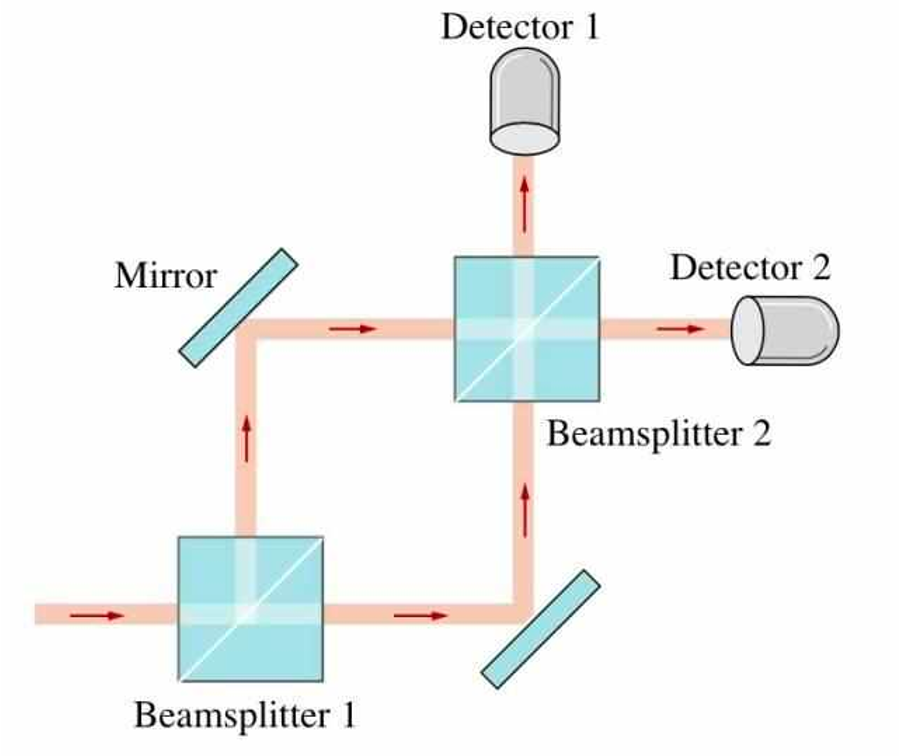
\includegraphics[width=0.45\textwidth]{figs/27.png}
    \end{center}
    {\Bullet}~结论: 物体总是处理叠加态\[\rs{\Psi}=c_1\rs{\Psi_1}+c_2\rs{\Psi_2}\]
\end{frame}

\begin{frame} 
    \frametitle{}
    \begin{tcolorbox4}[态叠加原理]
    {\Bullet}~如果 $\psi_1$ 、 $\psi_2$ 是粒子可能的态,那么它们的线性叠加
        $$ \Psi=c_1 \psi_1+ c_2\psi_2 $$
    也是粒子可能的态(叠加态)\\   
    {\Bullet}~如果粒子处于叠加态 $\Psi$,  
    那么测得粒子处在第$i$态 ($\psi_i$) 的概率为 $|c_i |^2$, 
    并且有  $$\sum_{i=1}^{N} |c_i|^2 =1$$
    \end{tcolorbox4}
    \Tips~ 量子位即薛定谔猫态,是一种$C^2$空间的叠加态
    \[\rs{S'cat}=\alpha\rs{died}+\beta\rs{alive} = \alpha\rs{0}+\beta\rs{1}\]
\end{frame} 

\begin{frame} 
    \frametitle{}
    {\Bullet} 叠加态是一种新的态,描述了体系的所有可能情况\\ \vspace{0.6em}
    {\Bullet} 量子比特就是由两个计算基矢态构成的叠加态,量子计算处理量子比特,即处理了体系所有可能的状态!
\end{frame} 

\section{2.量子纠缠态}

\begin{frame} 
    \frametitle{量子纠缠的定义}
    {\Bullet} ~双量子比特是单量子比特的张量积,可以写成四个计算基矢的叠加态:
    \[\rs{\psi} =(a_0\rs{0}+a_1\rs{1})\otimes (b_0\rs{0}+b_1\rs{1})=\alpha_{00}\rs{00}+\alpha_{01}\rs{01}+\alpha_{10}\rs{10}+\alpha_{11}\rs{11}\]
    {\Bullet} 定义:如果两个粒子的态函数不能写在单粒子态函数的张量积,则称为量子纠缠态
    \[\rs{\psi} \neq \rs{\psi_{1}} \otimes \rs{\psi_{2}} \]
\end{frame} 

\begin{frame} 
    \frametitle{}
    \例 [试确定下列态哪些是纠缠态]{}
    {\[ \Psi_1=\frac{\rs{00}+\rs{11}}{\sqrt{2}}; \qquad \Psi_2=\frac{\rs{01}+\rs{10}}{\sqrt{2}} ; \qquad \Psi_3=\frac{\rs{00}+\rs{10}}{\sqrt{2}} \]}
    \解~ $\Psi_3$不是纠缠态
    \[\begin{aligned}
        \Psi_3 &= \frac{\rs{00}+\rs{10}}{\sqrt{2}} \\
        &= \frac{\rs{0}+\rs{1}}{\sqrt{2}}\otimes \rs{0} \\
        &= \frac{\rs{0}+\rs{1}}{\sqrt{2}}\otimes (\rs{0}+0\rs{1}) \\
        &= \rs{\psi_{1}} \otimes \rs{\psi_{2}} 
    \end{aligned}\] 
\end{frame} 

\subsection{EPR效应}

\begin{frame} 
    \frametitle{EPR与量子纠缠}
    \begin{center}
        \includegraphics[width=0.9\textwidth]{figs/28.png}
    \end{center}
    {\Bullet} 是否存在超距离相互作用?\\
    {\Bullet} EPR态是纠缠态\[\rs{EPR}=\frac{\rs{\uparrow \downarrow }-\rs{\uparrow \downarrow }}{\sqrt{2}} = \frac{\rs{01 }-\rs{10 }}{\sqrt{2}} \]
\end{frame} 

\subsection{量子擦除实验}

\begin{frame}
    \frametitle{光子对的制备}
    激光与非线性光学介质发生作用时,产生多种非线性光学效应,比如:自发参量下转换(SPDC): 
    \begin{center}
        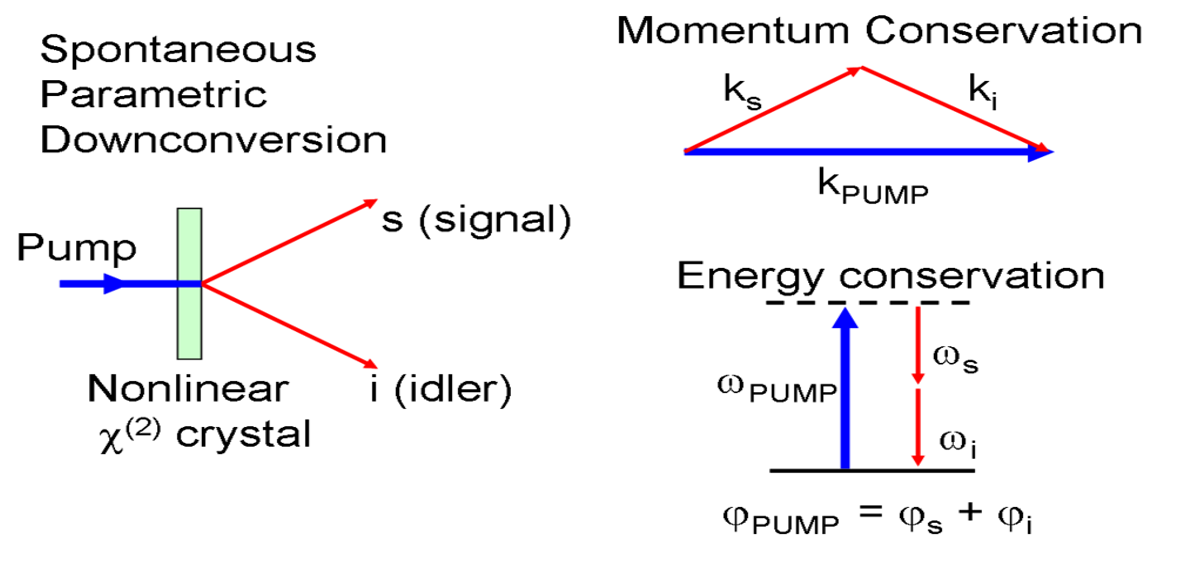
\includegraphics[width=0.7\textwidth]{figs/31.png}
    \end{center}
    每一个光子在被非线性晶体散射时,以一定概率转化为频率和波矢都不同的光子对(信号光子和闲置光子),
\end{frame}

\begin{frame}
    \frametitle{}
    \begin{center}
        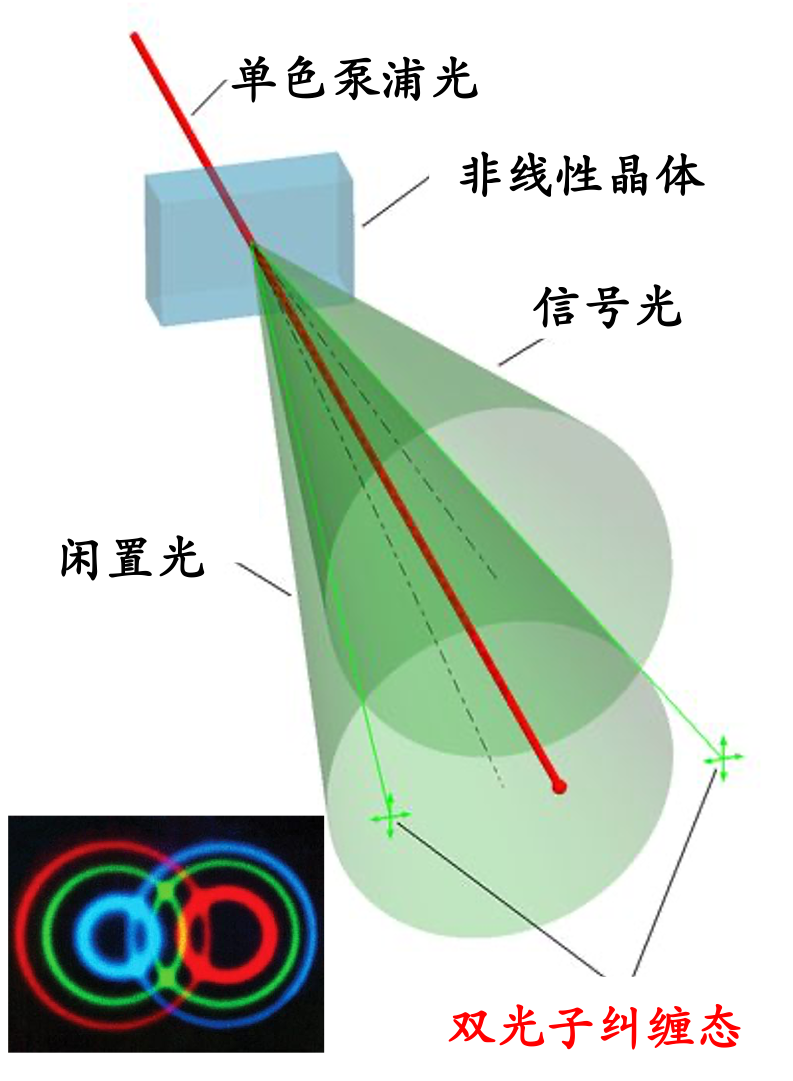
\includegraphics[width=0.42\textwidth]{figs/32.png}
    \end{center}
\end{frame}

\begin{frame}
    \frametitle{量子擦除实验}
    \begin{center}
        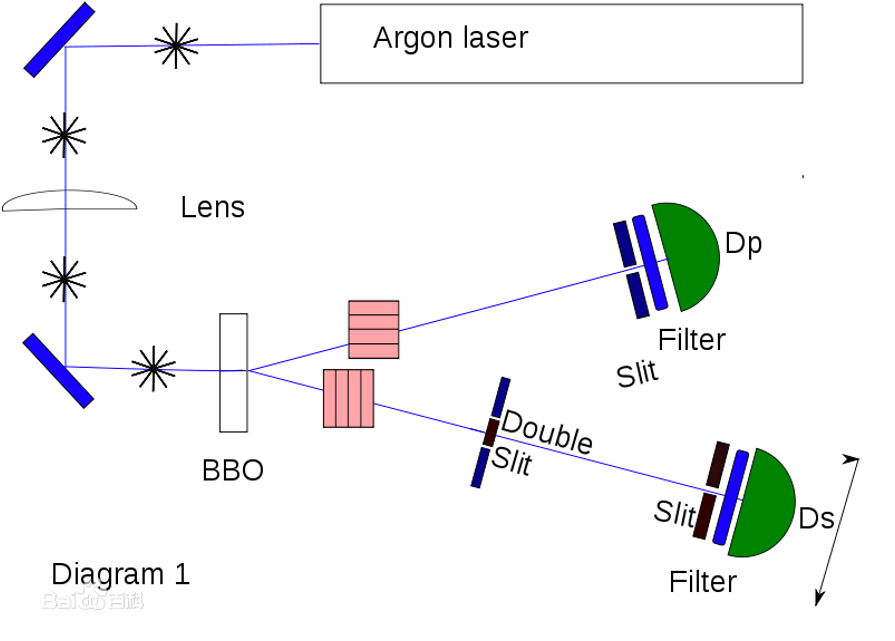
\includegraphics[width=0.55\textwidth]{figs/c1.png}
    \end{center}
    BBO晶体产生光子对,下路径光子过双缝形成干涉条纹.
\end{frame} 

\begin{frame}
    \frametitle{}
    \begin{center}
        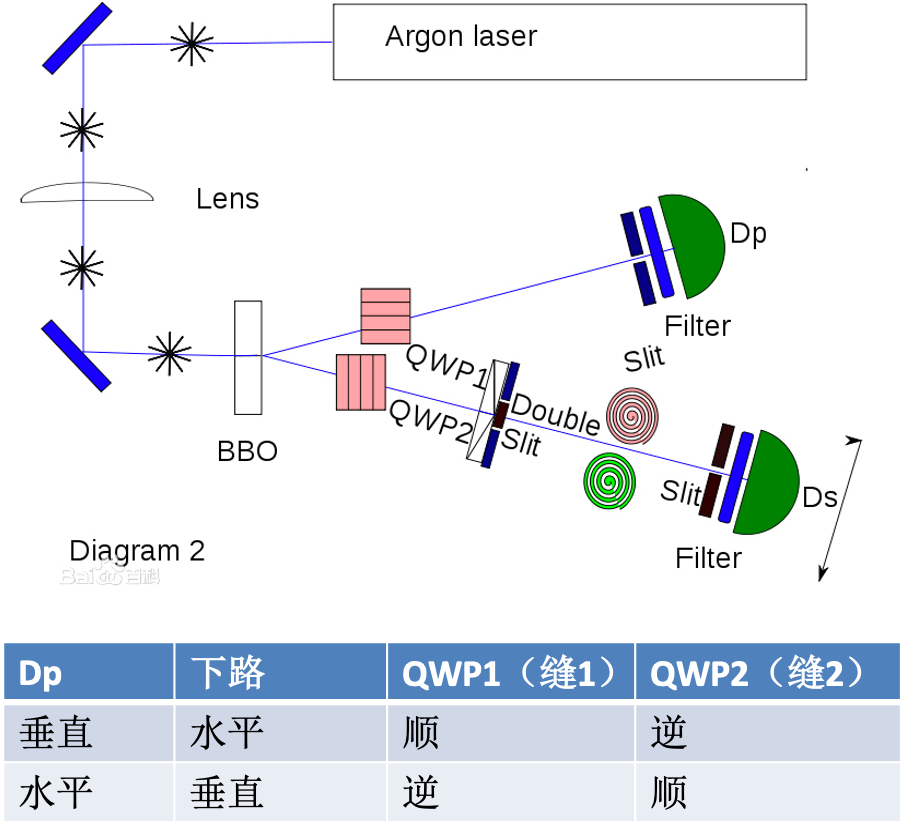
\includegraphics[width=0.6\textwidth]{figs/c2.png}
    \end{center}
    插入四分之一波片(QWP)进行路径测试,干涉条纹消失
\end{frame} 

\begin{frame}
    \frametitle{}
    \begin{center}
        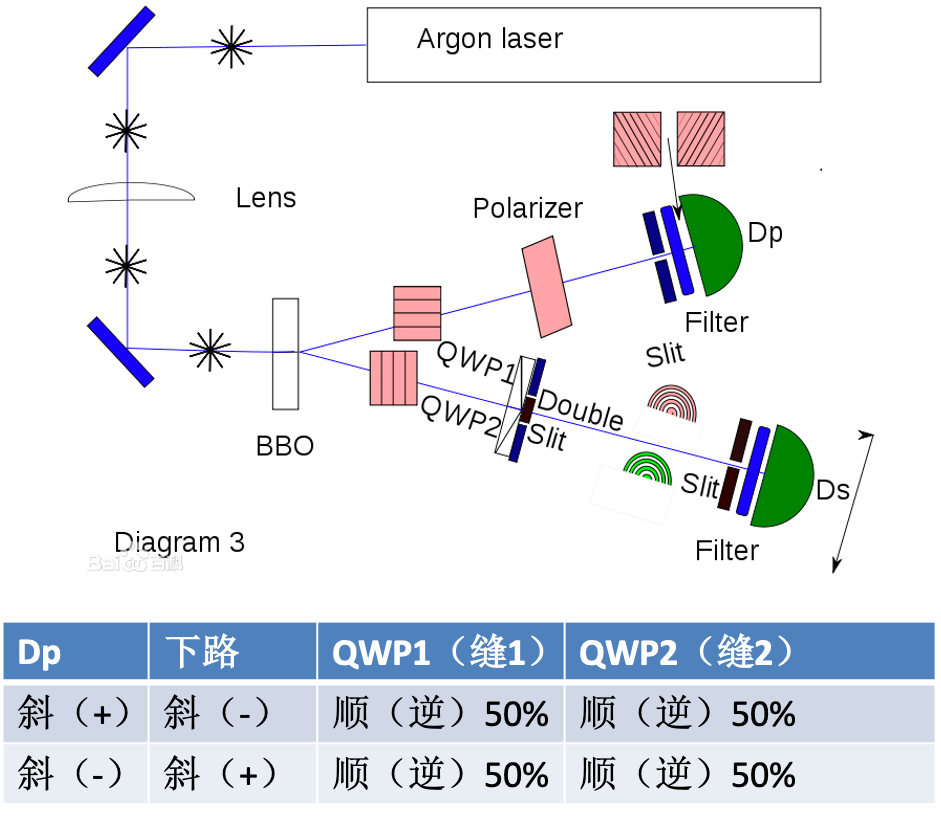
\includegraphics[width=0.6\textwidth]{figs/c3.png}
    \end{center}
    上光路径插入起偏器(Polarizer)下光路干涉条纹重新出现!
\end{frame} 

\begin{frame}
    问题: 起偏器改变的是上光子的偏振,为什么下光路干涉条纹重新出现?\\ \vspace{0.8em}
    结论: 自发参量下转换产生的是纠缠光子对,存在超距离相互作用
\end{frame} 

\begin{frame}
    \frametitle{贝尔(Bell)不等式}
    \begin{center}
        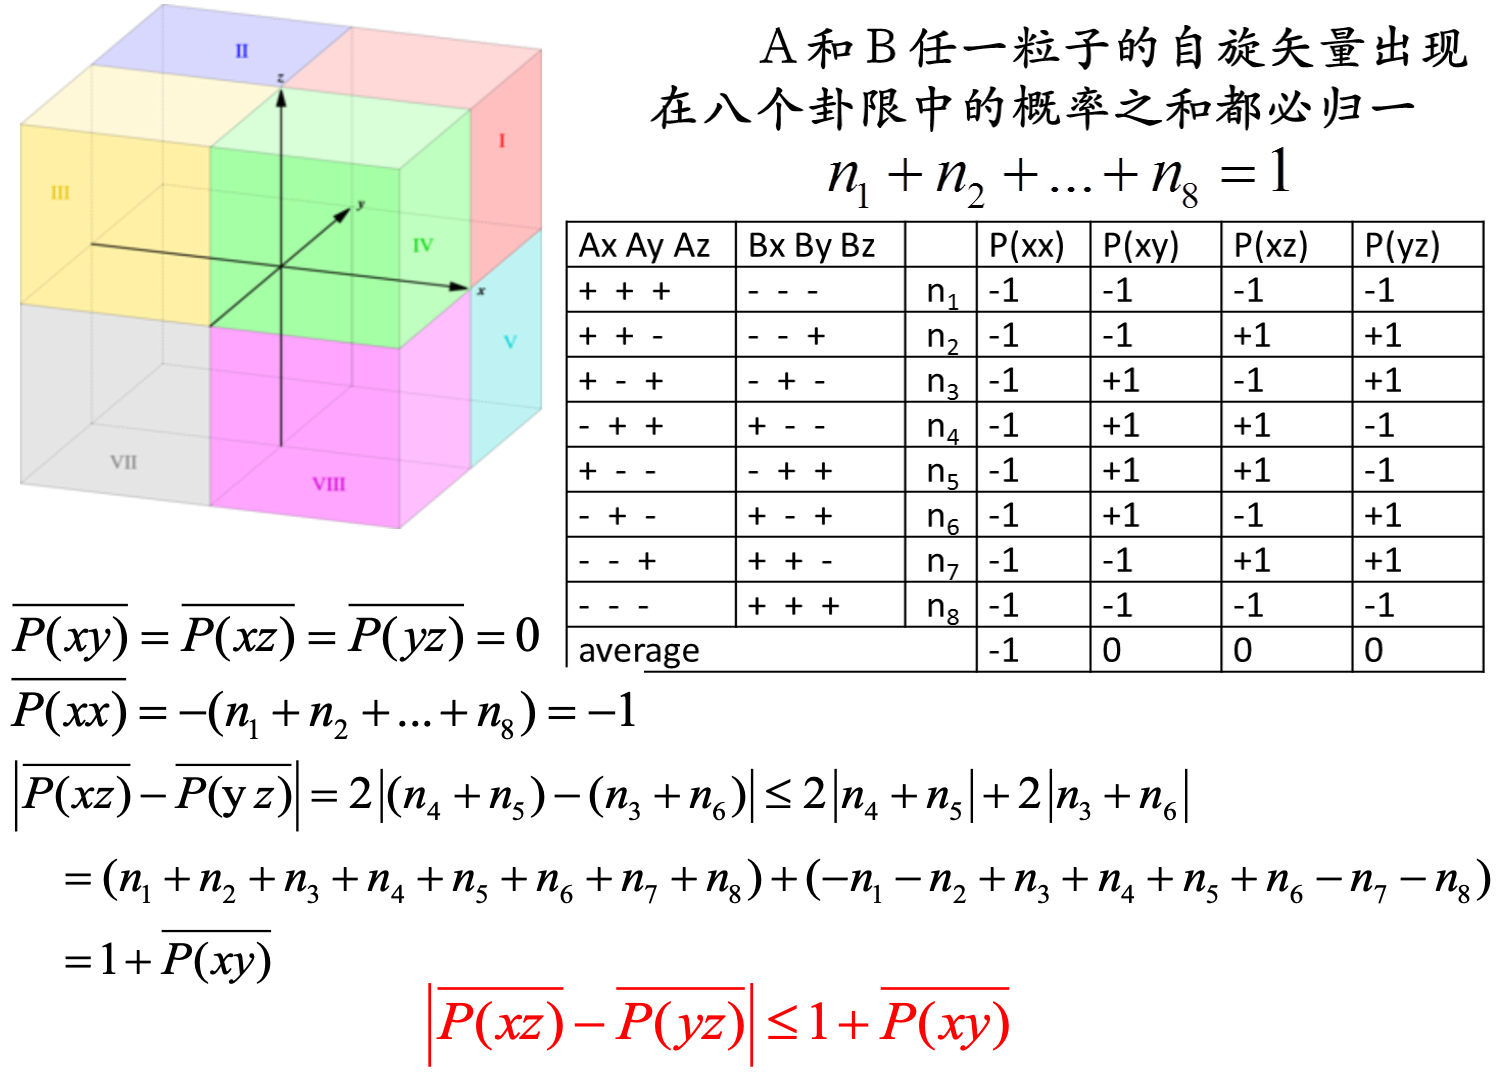
\includegraphics[width=0.75\textwidth]{figs/29.png}
    \end{center}
\end{frame} 

\subsection{贝尔纠缠态}

\begin{frame} 
    \frametitle{贝尔态}
    \[\rs{\beta_{00}}=\frac{\rs{00}+\rs{11}}{\sqrt{2}} =\frac{1}{\sqrt{2}} \begin{bmatrix}
        1 \\
        0 \\
        0 \\
        1
     \end{bmatrix} ; \qquad \rs{\beta_{01}}=\frac{\rs{00}-\rs{11}}{\sqrt{2}} = \frac{1}{\sqrt{2}} \begin{bmatrix}
        1 \\
        0 \\
        0 \\
        -1
     \end{bmatrix} \]
    \[\rs{\beta_{10}}=\frac{\rs{01}+\rs{10}}{\sqrt{2}} =\frac{1}{\sqrt{2}} \begin{bmatrix}
        0 \\
        1 \\
        1 \\
        0
     \end{bmatrix} ; \qquad \rs{\beta_{11}}=\frac{\rs{01}-\rs{10}}{\sqrt{2}} =\frac{1}{\sqrt{2}} \begin{bmatrix}
        0 \\
        1 \\
        -1 \\
        0
     \end{bmatrix} \]
\end{frame}


\begin{frame}
    \frametitle{}
    {\Bullet}试证明:贝尔态构成正交归一完备集\\ \vspace{1.0em}
    \证~归一性 \[\begin{aligned}
        \lr{\beta_{00}}{\beta_{00}} &= \frac{(\ls{00}+\ls{11})(\rs{00}+\rs{11})}{2} \\
        &= \frac{\lr{00}{00}+\lr{00}{11}+\lr{11}{00}+\lr{11}{11}}{2} \\
        &= \frac{1+0+0+1}{2} = 1 
    \end{aligned}\]
    正交性 \[\begin{aligned}
        \lr{\beta_{00}}{\beta_{01}} &= \frac{(\ls{00}+\ls{11})(\rs{00}-\rs{11})}{2} \\
        &= \frac{\lr{00}{00}+\lr{00}{11}+\lr{11}{00}-\lr{11}{11}}{2} \\
        &= \frac{1+0+0-1}{2} = 0 
    \end{aligned}\]
\end{frame}

\begin{frame}
    \frametitle{}
    {\Bullet}试证明:贝尔态是纠缠态\\ \vspace{1.0em}
    \证~用反正法,有单态
    \[ \rs{a} = a_0\rs{0}+a_1\rs{1}; \qquad \rs{b} = b_0\rs{0}+b_1\rs{1}\]
    设贝尔态可以写成单态的张量积
    \[ \begin{aligned}
    \beta_{00} &= \rs{a}\otimes \rs{b} \\
    \frac{\rs{01}+\rs{10}}{\sqrt{2}} &= (a_0\rs{0}+a_1\rs{1}) \otimes (b_0\rs{0}+b_1\rs{1}) \\
    &= a_0b_0\rs{00}+ a_0b_1\rs{01}+a_1b_0\rs{10}+a_1b_1\rs{11}
    \end{aligned}\]
    上式要成立,要求$a_0b_1\ne 0, a_1b_0 \ne 0; \quad \to \quad a_0b_1a_1b_0\ne 0$ \\
    上式要成立,要求$a_0b_0= 0, a_1b_1 = 0; \quad \to \quad a_0b_1a_1b_0= 0$ \\
    自相矛盾,证毕!
\end{frame}

\begin{frame}
    \frametitle{}
    {\Bullet}试证明如下量子线路,可以生成Bell态:
    \[\rs{00}\to\rs{\beta_{00}}; \rs{01}\to\rs{\beta_{01}}; \rs{10}\to\rs{\beta_{10}}; \rs{11}\to\rs{\beta_{11}}\]
    \begin{center}
        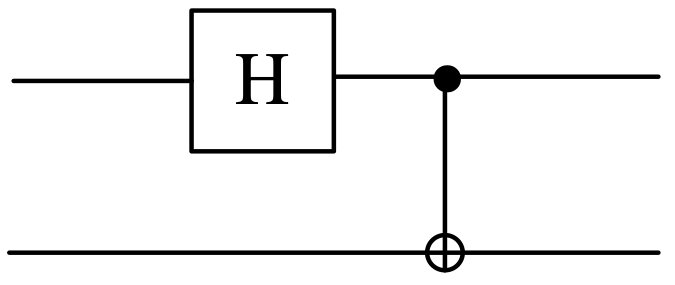
\includegraphics[width=0.35\textwidth]{figs/30.png}
    \end{center}
    \证~设输入为$\rs{00}$ \\
    \begin{itemize}
        \item $H\rs{00}=H\rs{0}\rs{0}=\Pstate\rs{0}=\dfrac{\rs{00}+\rs{10}}{\sqrt{2}}$ 
        \item $CNOT\dfrac{\rs{00}+\rs{10}}{\sqrt{2}}=\dfrac{\rs{00}+\rs{11}}{\sqrt{2}}=\beta_{00}$
    \end{itemize}
    证毕!
\end{frame}

\subsection{多粒子纠缠态}

\begin{frame}{三粒子纠缠态}
    试证明如下三粒子态都是纠缠态
    \[ (1) \rs{GHZ}=\frac{1}{\sqrt{2}}(\rs{000}+\rs{111}); \quad (2) \rs{W}=\frac{1}{\sqrt{3}}(\rs{001}+\rs{010}+\rs{100})\] 
    \[(3) \rs{\Psi}=\frac{1}{2}(\rs{010}+\rs{011}+\rs{100}+\rs{101})\]
    \证 
    \[ \begin{aligned}
        \rs{\Psi}&=\frac{1}{2}(\rs{010}+\rs{011}+\rs{100}+\rs{101}) \\
         &=(\frac{\rs{01}+\rs{10}}{\sqrt{2}})(\Pstate) \\
         &=\rs{\beta_{10}}\otimes\rs{+}
    \end{aligned}\]
    即,前两个粒子处于纠缠态
\end{frame}

\begin{frame}
    \frametitle{}
    \begin{tcolorbox3}[专题:光子叠加态与纠缠光子对]
        (1)产生光子叠加态的方案 \\
        (2)产生纠缠光子对的方案\\
        (3)光子对可以产生哪些自由度上的纠缠
    \end{tcolorbox3}
\end{frame}